% !TeX program = lualatex
% !TeX encoding = utf8
% !TeX spellcheck = uk_UA
% !BIB program = bibler

\documentclass[onlytextwidth]{beamer}
\usetheme{Electromagnetism}



\usepackage{Electromagnetism}
\hypersetup{
  colorlinks=true,
  linkcolor=cyan,  % Цвет для внутренних ссылок
  urlcolor=red,    % Цвет для URL
  citecolor=blue   % Цвет для библиографических ссылок
}




%============================================================================
\title[Лекції електрики та магнетизму]{\huge\bfseries Провідники \\ в електричному полі}
\subtitle{Лекції з електрики та магнетизму}
\author{Пономаренко С. М.}
\date{}
%============================================================================
\graphicspath{{pictures/}}
\begin{document}


\begin{frame}[plain]
	\maketitle
	%	\tikz[remember picture,overlay] \node[opacity=0.7,inner sep=0pt,
	%		anchor=north west] at (current page.north
	%	west){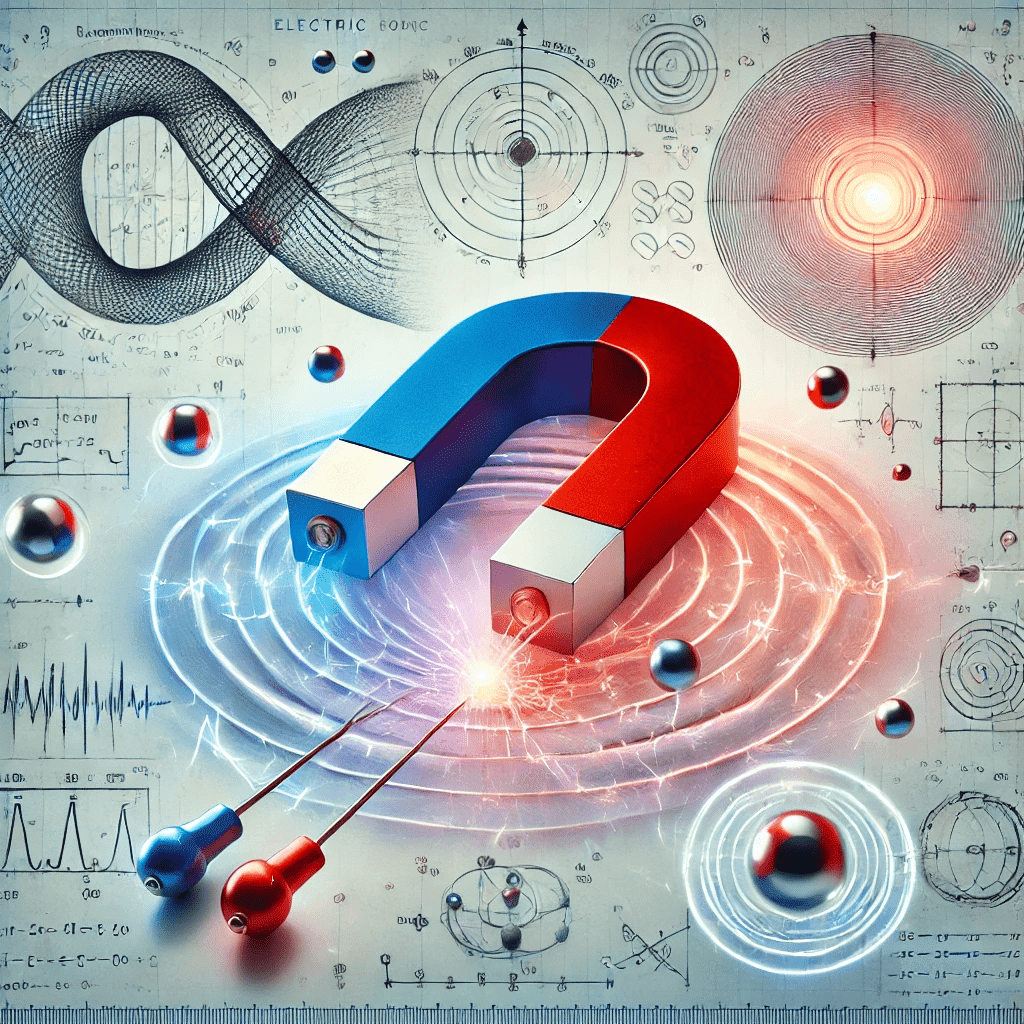
\includegraphics[width=2cm]{EMInteractions}};
\end{frame}

% ============================== Слайд ## ===================================
\begin{frame}{Зміст лекції}{}
       \tableofcontents
\end{frame}
% ===========================================================================

%% --------------------------------------------------------
\section{Структура провідників}
%% --------------------------------------------------------


% ============================== Слайд ## ===================================
\begin{frame}{Природа носіїв струму в металах}{Досліди Толмена та Стюарта}\small
	\begin{block}{}\justifying
		У 1916 р. американський фізик Р. Толмен (1881-1948) і шотландський фізик Т. Стюарт виконали
		кількісні виміри, які неспростовно довели, що струм у металевих провідниках зумовлений рухом
		вільних електронів.
	\end{block}
	%\begin{onlyenv}<1>
	\begin{columns}
		\begin{column}{0.65\linewidth}
			\begin{block}{}\justifying
				У цих дослідах котушку з великим числом витків тонкого дроту підключали до
				гальванометра і приводили в швидке обертання навколо своєї осі. Під час різкого
				гальмування котушки в колі виникав короткочасний струм, зумовлений інерцією носіїв
				заряду. За напрямком відхилення стрілки гальванометра було встановлено, що
				\alert{електричний струм створюють негативно заряджені частинки}. При цьому
				експериментально був отриманий питомий заряд носіїв $q/m$ близький до питомого
				заряду електрона, отриманого з інших дослідів. Так було експериментально доведено,
				що носіями вільних зарядів у металах є електрони.
			\end{block}
		\end{column}
		\hfill
		\begin{column}{0.3\linewidth}\centering
			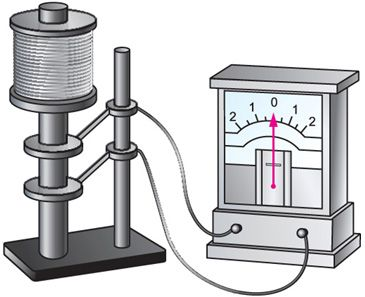
\includegraphics[width=\linewidth]{exptommstuart}
			\begin{block}{}\centering
				Установка Толмена і Стюарта
			\end{block}
		\end{column}
	\end{columns}
	\begin{block}{}
		\href{https://www.youtube.com/watch?v=nVwquffMk44}{\color{blue}Відеодемотнстрація дослідів}
	\end{block}
\end{frame}
% ===========================================================================




% ============================== Слайд ## ===================================
\begin{frame}[fragile]{Структура провідників}{}
	\begin{block}{}\justifying
		Провідниками називають речовини в структурі яких є вільні заряди (електрони в металах,
		наприклад), які можуть переміщуватися під дією як завгодно слабких полів.
	\end{block}
	\tikzstyle{charge+}=[ball color=red!50, text=white]
	\tikzstyle{charge-}=[ball color=blue!50, text=white]
	\tikzstyle{metal}=[top color=black!15,bottom color=black!25,middle color=black!5,shading
	angle=10]

	% CONDUCTION MODEL
	\def\R{0.21} % ion radius
	\def\a{0.90} % scale
	\def\Rx{0.2*\a*\Ny}
	\def\Ry{0.5*\a*\Ny}
	\def\Nx{6} % number of ions columns
	\def\Ny{3} % number of ions rows
	\def\L{\a*(\Nx-1)} % length
	\NewDocumentCommand{\electron}{ m m m}{
		\node[charge-,draw=black,circle,fill,inner sep=0.8,scale=0.5,line width=0.3] (e) at
		({#1*\a},{#2*\a}) {$-$};
		\draw[->,green!60!black] (e) --++ (#3*0.7*\a);
	}
	\begin{center}
		\begin{tikzpicture}[>=latex]

			% \fill[metal] (0,{-\Ry}) arc (270:90:{\Rx} and {\Ry}) --++ ({\L},0) arc (90:-90:{\Rx} and {\Ry});
			%  \draw[black!80] (0,{-\Ry}) arc (270:90:{\Rx} and {\Ry});
			%  \draw[black!80,dashed] ({\L},{-\Ry}) arc (270:90:{\Rx} and {\Ry});
			%
			% IONS
			\foreach \j [evaluate={\y=\a*(\j-\Ny/2-0.5);}] in {1,...,\Ny}{
					\foreach \i in {1,...,\Nx}{ %[evaluate={\x=\j*\a;}]
							\draw[charge+] ({(\i-1)*\a},\y) circle (\R) node[scale=1.4*\a,inner
									sep=1] {$+$};
						}
				}

			%%%%%%%%%%%%%%%%%%%%%%%%%%%%%%%%% 0
			\electron{-0.25}{ 0.55}{ -99:0.6}
			%%%%%%%%%%%%%%%%%%%%%%%%%%%%%%%%% 1
			\electron{ 0.10}{-0.55}{ 210:0.7}
			\electron{ 0.40}{ 0.35}{ 120:0.5}
			\electron{ 0.55}{ 1.30}{  10:0.6}
			%%%%%%%%%%%%%%%%%%%%%%%%%%%%%%%%% 2
			\electron{ 0.65}{-1.30}{-160:0.6}
			\electron{ 1.30}{-0.40}{  30:0.6}
			\electron{ 1.15}{ 0.40}{ 210:0.6}
			%%%%%%%%%%%%%%%%%%%%%%%%%%%%%%%%% 3
			\electron{ 2.35}{-0.70}{ -40:0.6}
			\electron{ 2.05}{ 0.55}{ -40:0.6}
			\electron{ 2.30}{ 1.30}{ -75:0.7}
			%%%%%%%%%%%%%%%%%%%%%%%%%%%%%%%%% 4
			\electron{ 3.30}{-1.30}{  20:0.5}
			\electron{ 3.40}{ 1.10}{-110:0.6}
			%%%%%%%%%%%%%%%%%%%%%%%%%%%%%%%%% 5
			\electron{ 3.38}{-0.45}{ -40:0.6}
			\electron{ 3.90}{ 0.40}{ 175:0.7}
			\electron{ 4.35}{ 1.30}{ -20:0.6}
			%%%%%%%%%%%%%%%%%%%%%%%%%%%%%%%%% 6
			\electron{ 4.45}{-0.95}{ -80:0.6}
			\electron{ 5.25}{-0.40}{  45:0.5}
			\electron{ 4.60}{-0.05}{-110:0.6}
			\electron{ 5.30}{ 0.60}{-150:0.6}
			%%%%%%%%%%%%%%%%%%%%%%%%%%%%%%%%%

			%  \draw[black!80] (0,{-\Ry}) arc (-90:90:{\Rx} and {\Ry}) --++ ({\L},0) arc (90:-90:{\Rx} and
			%  {\Ry}) -- cycle;
		\end{tikzpicture}
	\end{center}

	\begin{block}{}\justifying\small
		Електронні оболонки атомів, що складають кристалічну решітку металів, сильно
		перекриваються, внаслідок чого не можна вказати, біля якого іона локалізовано той чи інший
		\alert{електрон валентної оболонки}, --- вони легко перетікають від одного іона до іншого,
		і, в цьому разі, кажуть, що \alert{електрони колективівізовані}. Іони являють собою ядра і
		електрони внутрішніх оболонок, які сильно локалізовані. Електрони, які делокалізовані
		вільно переміщаються по кристалу. Саме вільні електрони відповідають за багато фізичних і,
		особливо, транспортних властивостей металів.
	\end{block}

\end{frame}
% ===========================================================================




%% --------------------------------------------------------
\section{Провідник в полі}
%% --------------------------------------------------------




% ============================== Слайд ## ===================================
\begin{frame}{Провідник в полі}{}
	\begin{columns}
		\begin{column}{0.6\linewidth}
			\begin{block}{}\justifying\small
				Якщо провідник потрапляє в поле, електрони в ньому починають рухатися проти поля.
				На одній частині поверхні провідника виступає негативний заряд, ця поверхня стає
				збагаченою електронами. На протилежній частині поверхні
				електронів виявляється дещо менше, ніж потрібно для нейтралізації позитивного
				іонного заряду кристалічної решітки, і ця частина поверхні виявляється зарядженою
				позитивно. Позитивна і негативна частини поверхні створюють своє власне поле, за
				напрямком протилежне зовнішньому. Обидва поля --- зовнішнє $\Efield_\text{ex}$ і
				поле власних     поверхневих зарядів провідника ($\Efield_\text{in}$) точно
				компенсують одне одне в усіх точках усередині і     на поверхні.
				%
				%                Якби в якій-небудь
				%                ділянці провідника поля $\Efield_\text{ex}$ і $\Efield_\text{in}$
				%не компенсували
				%                одне одного, то в цій ділянці на електрони діяла б сила і йшов би
				%струм.
				%                Відсутність струму означає повну компенсацію полів.
			\end{block}
		\end{column}
		\begin{column}{0.4\linewidth}
			\begin{overprint}
				\onslide<1>
				\begin{center}
					\begin{tikzpicture}[>=latex, scale=0.7]
						\clip (-3, -2.6) rectangle (3,2.6);
						\pgfmathsetseed{9}
						\draw[ball color=gray!5, name path=metall, smooth] plot [smooth cycle,
								samples=8,domain={1:10}]
						(\x*360/10+5*rnd:0.5cm+1cm*rnd);


						\foreach[] \y in {-3,...,3} {
								\draw[->, red] (-3, 0.6*\y) -- ++(6, 0);
							}

						\foreach[count=\c] \y in {-3,...,4} {
								\path[name path global=Q\c] (-2, 0.25*\y) -- ++(4, 0);
							}

						\foreach \c in {1,...,7} {
								\path[name intersections={of=metall and Q\c}]  (intersection-1)
								node[anchor=center, right,
									text=blue, font=\tiny] (A\c) {$-$}
								(intersection-2)  node  [anchor=center, left,
									text=red, 							font=\tiny] (B\c) {$+$} ;
								\draw[->, red, densely dashed] (B\c) -- (A\c);
							};
						%			\path (-3,2.23) node (x) {} -- ++(6,0);
					\end{tikzpicture}
				\end{center}
				\onslide<2->
				\begin{center}
					\begin{tikzpicture}[>=latex, scale=0.7]
						\pgfmathsetseed{9}
						\draw[ball color=gray!5, name path=metall, smooth] plot [smooth cycle,
								samples=8,domain={1:10}]
						(\x*360/10+5*rnd:0.5cm+1cm*rnd);

						\foreach[count=\c] \y in {-3,...,4} {
								\path[name path global=Q\c] (-2, 0.25*\y) -- ++(4, 0);
							}

						\foreach \c in {1,...,8} {
								\path[name intersections={of=metall and Q\c}]  (intersection-1)
								coordinate (A\c)
								node[anchor=center, right,
										text=blue, font=\tiny] {$-$}
								(intersection-2) coordinate (B\c) node [anchor=center, left,
										text=red, ,
										font=\tiny] {$+$} ;
							};

						\begin{scope}
							\clip (-3, -2.6) rectangle (3,2.6);
							\draw[red, midarrowR] (A1) to [out=-135, in=-10] ++(-3, -0.7);
							\draw[red, midarrowR] (A2) to [out=-145, in=0] ++(-3, -0.6);
							\draw[red, midarrowR] (A3) to [out=-155, in=0] ++(-3, -0.4);
							\draw[red, midarrowR] (A4) to [out=180, in=0] ++(-3, 0);
							\draw[red, midarrowR] (A5) to [out=140, in=0] ++(-3, 0.4);
							\draw[red, midarrowR] (A6) to [out=140, in=0] ++(-3, 0.6);
							\draw[red, midarrowR] (A7) to [out=150, in=0] ++(-3, 0.7);
							\draw[red, midarrowR] (A8) to [out=140, in=-15] ++(-2.5, 0.9);

							\draw[red, midarrow] (B1) to [out=-45, in=180] ++(3, -1);
							\draw[red, midarrow] (B2) to [out=-40, in=180] ++(3, -0.9);
							\draw[red, midarrow] (B3) to [out=-40, in=180] ++(3, -0.8);
							\draw[red, midarrow] (B4) to [out=-30, in=180] ++(3, -0.7);
							\draw[red, midarrow] (B5) to [out=40, in=180] ++(3, 0.4);
							\draw[red, midarrow] (B6) to [out=40, in=190] ++(3, 0.8);
							\draw[red, midarrow] (B7) to [out=40, in=185] ++(3, 0.9);
							\draw[red, midarrow] (B8) to [out=40, in=200] ++(3, 1.2);

							\draw[red, midarrow] ([shift={(-2, -1.2)}]A1) to[out=20, in=160]
							([shift={(3,
										-1.7)}]B1);
							\draw[red, midarrow] ([shift={(-2, +1.8)}]A6) to[out=-20, in=-160]
							([shift={(3,
										+2.3)}]B6);
						\end{scope}
						%			\path (-3,-2.6) node (x) {} -- ++(6,0);
					\end{tikzpicture}
				\end{center}
			\end{overprint}
		\end{column}
	\end{columns}
	\begin{overprint}
		\onslide<1-2>
		\begin{block}{}\justifying
			\alert{В стаціонарному стані}, коли немає струмів, в \alert{об'ємі
				провідника результуюче електричне поле}:
			\begin{equation*}
				\Efield = 0
			\end{equation*}
			Струм буде текти доти, доки заряди не розташуються так, щоб поле було
			відсутнє усюди в об'ємі провідника.
		\end{block}
		\onslide<3>
		\begin{block}{}\justifying
			З теореми Гаусса
			\begin{equation*}
				\Efield = 0\ {\color{red}\Rightarrow}\ \rho = \frac1{4\pi} \Div\Efield\
				{\color{red}\Rightarrow}\ \rho = 0,
			\end{equation*}
			об'ємна густина зарядів у провіднику дорівнює нулю, \alert{вільні заряди можуть
				розташовуватися тільки на поверхні}.
		\end{block}
		\onslide<4>
		\begin{block}{}
			Граничні умови
			\begin{align*}
				E_n      & = 4\pi\sigma, \\
				E_{\tau} & = 0
			\end{align*}
			показують, що \alert{силові лінії входять перпендикулярно в провідник}.
		\end{block}
        \onslide<5>
        \begin{alertblock}{}
            Поверхня провідника є еквіпотенціальною поверхнею! Потенціал в об'ємі провідника
            постійний і дорівнює потенціалу на його поверхні:
            \begin{equation*}
                \phi_S = \phi_V = \const.
            \end{equation*}
        \end{alertblock}
	\end{overprint}
\end{frame}
% ===========================================================================




%% --------------------------------------------------------
\section{Поле в порожнині провідника}
%% --------------------------------------------------------




% ============================== Слайд ## ===================================
\begin{frame}{Поле в порожнині провідника}
	\begin{block}{}\justifying
		Зовнішні заряди, зокрема заряди на зовнішній поверхні провідника, не створюють у товщі
		провідника жодного електричного поля. \alert{Чи будуть з'являтись заряди на внутрішній поверзні
			провідника, в якому є порожнина?}
	\end{block}
	\begin{columns}
		\begin{column}{0.7\linewidth}
			\begin{overprint}
				\onslide<1>
				\begin{block}{}\justifying
					Якщо в \alert{порожнині незарядженого провідника є заряд}, то на внутрішній
					поверхні оболонки будуть створюватись індуковані заряди протилежного знаку. На
					зовнішній оболонці заряд розподілиться по поверхні. На основі теореми Гаусса заряд
					на зовнішній поверхні буде дорівнювати заряду в порожнині.
				\end{block}
				\onslide<2>
				\begin{block}{}\justifying
					Якщо в \alert{порожнині провідника немає зарядів}, то на внутрішній поверхні
					оболонки зарядженого провідника індукованих зарядів не буде, а поле в порожнині
					дорівнює нулю. Провідна оболонка повністю екранує поле всіх зарядів, що знаходяться
					поза оболонкою.
					%На цьому заснований \alert{електростатичний захист} --- екранування  тіл,
					%наприклад вимірювальних приладів, від впливу зовнішніх електростатичних полів.
				\end{block}
			\end{overprint}
		\end{column}
		\begin{column}{0.3\linewidth}\centering
			\begin{overprint}\centering
				\onslide<1>
				\begin{tikzpicture}[>=latex,
		draw charges/.style={decorate,decoration={
						markings,mark=between positions 0 and
						1 step
						.05 with
							{\node[text=red, font=\tiny] at (0,0) {$+$};},
					}
			}
	]
		\pgfmathsetseed{55}
		\clip[smooth, scale=1.1] plot
			[smooth cycle,
				samples=8,domain={1:10}]
		(\x*360/10+5*rnd:1cm+1cm*rnd);
	\begin{scope}

		\pgfmathsetseed{55}
		\draw[ball color=gray!5, name path=metall, smooth] plot
			[smooth cycle,
				samples=8,domain={1:10}]
		(\x*360/10+5*rnd:1cm+1cm*rnd);
		\pgfmathsetseed{55}
		\draw[fill=white=gray!5, name path=metall, smooth, scale=0.5, yshift=0.5cm, name path
			global=cavity] plot
			[smooth cycle,
				samples=8,domain={1:10}]
		(\x*360/10+5*rnd:1cm+1cm*rnd);
		\pgfmathsetseed{55}
		\path[smooth, postaction=draw charges, scale=0.95]
		plot
			[smooth cycle,
				samples=8,domain={1:10}]
		(\x*360/10+5*rnd:1cm+1cm*rnd);
	\end{scope}
	\foreach[count=\c] \r in {0.5,0.8,...,2.5} {
			\path[name path global=charge\c] (0, -0.5) circle[x radius=\r, y radius=0.5*\r];
		}
	\foreach \c in {1,...,6} {
			\path[name intersections={of=cavity and charge\c}]  (intersection-1)
			node[anchor=east,
				text=blue, font=\tiny, inner sep=1pt] (A\c) {$-$}
			(intersection-2)  node  [anchor=west, inner sep=1pt,
				text=blue, font=\tiny] (B\c) {$-$} ;
		};
        \node[circle, inner sep=1pt, ball color=red, text=white, font=\scriptsize] (Q) at (-0.25,0)
        {$+$};
        \draw[midarrowR, red] (A1) -- (Q);
        \draw[midarrowR, red] (A2) -- (Q);
        \draw[midarrowR, red] (A3) -- (Q);
        \draw[midarrowR, red] (A4) -- (Q);
        \draw[midarrowR, red] (A5) to[out=-10] (Q);
        \draw[midarrowR, red] (A6) to[bend left] (Q);

        \draw[midarrow, red] (Q) to[out=75, in=135] (B6);
        \draw[midarrow, red] (Q) to[out=35, in=195] (B5);
        \draw[midarrow, red] (Q) to[out=0, in=205] (B4);
        \draw[midarrow, red] (Q) to[out=-30, in=200] (B3);
        \draw[midarrow, red] (Q) to[out=-70, in=180] (B2);
\end{tikzpicture}
				\onslide<2>
				\begin{tikzpicture}[>=latex,
		draw charges/.style={decorate,decoration={
						markings,mark=between positions 0 and
						1 step
						.05 with
							{\node[text=red, font=\tiny] at (0,0) {$+$};},
					}
			}
	]
		\pgfmathsetseed{55}
		\clip[smooth, scale=1.1] plot
			[smooth cycle,
				samples=8,domain={1:10}]
		(\x*360/10+5*rnd:1cm+1cm*rnd);
	\begin{scope}
		\pgfmathsetseed{55}
		\draw[ball color=gray!5, name path=metall, smooth] plot
			[smooth cycle,
				samples=8,domain={1:10}]
		(\x*360/10+5*rnd:1cm+1cm*rnd);
		\pgfmathsetseed{55}
		\draw[fill=white=gray!5, name path=metall, smooth, scale=0.5, yshift=0.5cm, name path
			global=cavity] plot
			[smooth cycle,
				samples=8,domain={1:10}]
		(\x*360/10+5*rnd:1cm+1cm*rnd);
		\pgfmathsetseed{55}
		\path[smooth, postaction=draw charges, scale=0.95]
		plot
			[smooth cycle,
				samples=8,domain={1:10}]
		(\x*360/10+5*rnd:1cm+1cm*rnd);
	\end{scope}
	\foreach[count=\c] \r in {0.5,0.8,...,2.5} {
			\path[name path global=charge\c] (0, -0.5) circle[x radius=\r, y radius=0.5*\r];
		}
	\draw[black, ->, densely dashed] (0,-0.5) [partial ellipse=125:50:1 and 0.5] node[pos=0.5,
	above, text=red]
	{?};
	\draw[black, densely dashed] (0,-0.5) [partial ellipse=45:-230:1 and 0.5];
	\foreach \c in {1,...,4} {
			\path[name intersections={of=cavity and charge\c}]  (intersection-1)
			node[anchor=east,
				text=blue, font=\tiny, inner sep=1pt] (A\c) {$-$}
			(intersection-2)  node  [anchor=west, inner sep=1pt,
				text=red, font=\tiny] (B\c) {$+$} ;
		};
\end{tikzpicture}
			\end{overprint}
		\end{column}
	\end{columns}
	\begin{alertblock}{}\justifying
		Замкнута провідна оболонка розділяє весь простір на внутрішню і зовнішню частини, які в
		електричному відношенні абсолютно \alert{не залежать одна від одної}.
	\end{alertblock}
\end{frame}
% ===========================================================================





% ============================== Слайд ## ===================================
\begin{frame}{Експериментальна перевірка закону Кулона}{}\small
\begin{block}{}\justifying
    На основі того факту, що \alert{заряди витісняються на поверхню зарядженого провідника} засновано \alert{експеримент по перевірці закону обернених
    квадратів в законі Кулона}. Якщо закон взаємодії точкових зарядів відрізняється від закону оберненого квадрату на малу величину:
\begin{equation*}
F = \frac{q_1 q_2}{r^{2 + \epsilon}},\quad \text{де}\ |\epsilon| \ll 1.
\end{equation*}
то у провіднику виникає ненульова об'ємна густина заряду.
\end{block}
\begin{columns}
	\begin{column}{0.4\linewidth}
         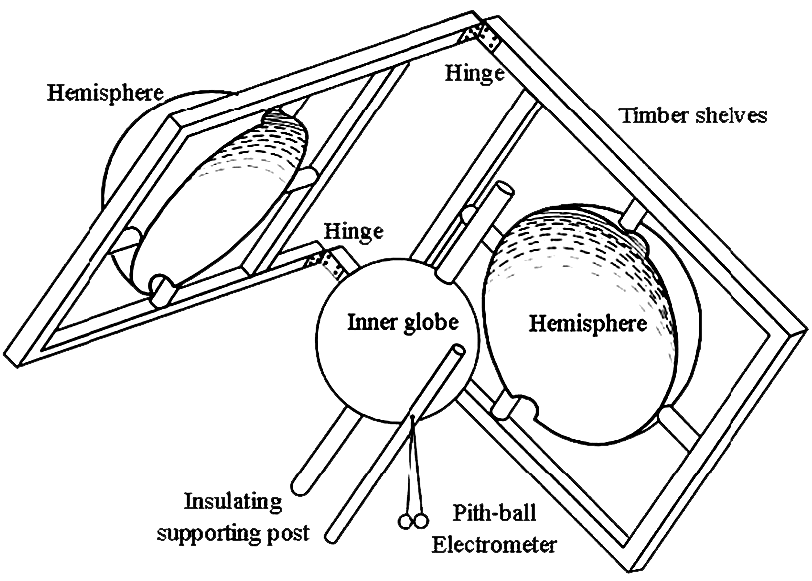
\includegraphics[width=\linewidth]{cavindesh_exp}
	\end{column}
	\begin{column}{0.59\linewidth}
 \begin{block}{}\justifying\footnotesize
    Це було використано для отримання обмеження на $\epsilon$. На попередньо заряджену провідну кулю накладали дві провідні напівсфери, які
щільно прилягали одна до одної, утворюючи майже суцільну поверхню. У цій системі, у разі кулонівської взаємодії ($\epsilon = 0$), весь заряд
переходить на зовнішні напівсфери. Якщо ж $\epsilon \neq 0$, всередині кулі залишається заряд (тим менший, чим менше $\epsilon$), який можна
виміряти за допомогою чутливого електрометра після зняття напівсфер. Цей експеримент неодноразово повторювався із поступовим підвищенням точності. У
1983 році було отримано обмеження:
\begin{equation*}
|\epsilon| < 10^{-16} \text{–} 10^{-17}.
\end{equation*}
\end{block}
	\end{column}
\end{columns}

\end{frame}
% ===========================================================================




%% --------------------------------------------------------
\subsection{Електростатичний захист}
%% --------------------------------------------------------



% ============================== Слайд ## ===================================
\begin{frame}{Електростатичний захист}
	\begin{block}{}\justifying
		Електростатичний захист --- явище, згідно з яким, можна екранувати електричне поле,
		<<сховавшись>> від нього всередині замкненої металевої оболонки. На практиці
		використовують сітку.
	\end{block}
	\begin{columns}
		\begin{column}{0.49\linewidth}\centering
			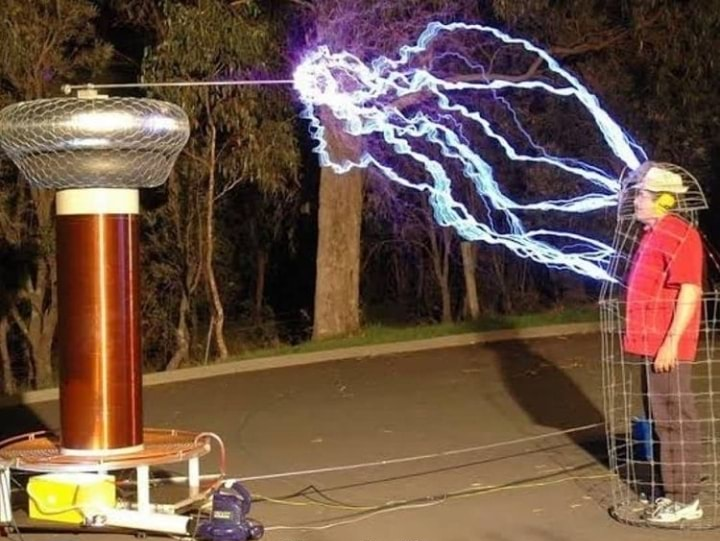
\includegraphics[width=0.9\linewidth]{FaradayCage}
		\end{column}
		\begin{column}{0.5\linewidth}
			\begin{block}{}\small\justifying
				Явище було відкрито Майклом Фарадеєм 1836 року. Він звернув увагу, що зовнішнє
				електричне поле не може потрапити всередину металевої клітки. Електростатичний
				захист потрібен там, де необхідно екранувати електроприлади від зовнішніх
				електричних полів (наприклад, в блоках живлення, материнській платі комп'ютера,
				лабораторному обладнанні). Ці прилади поміщаються в металевий корпус, який захищає
				їх від зовнішніх електричних перешкод.
			\end{block}
		\end{column}
	\end{columns}
	\begin{block}{}
		\href{https://www.youtube.com/watch?v=jsBmv3-i2g0}{Відео: клітка Фарадея}
	\end{block}
\end{frame}
% ===========================================================================


%% --------------------------------------------------------
\subsection{Електростатичний генератор Ван-де-Граафа}
%% --------------------------------------------------------



% ============================== Слайд ## ===================================
\begin{frame}{Електростатичний генератор Ван-де-Граафа}{}
	\begin{block}{}
		Генератор Ван де Граафа --- електростатичний генератор в якому використовуються властивості
		циліндра Фарадея для створення високої напруги. Таким методом можна досягнути напруги до
		кількох мегавольт.
	\end{block}
	\begin{columns}
		\begin{column}{0.7\linewidth}
			\begin{block}{}\justifying
				Діелектрична стрічка обертається між двох роликів. Знизу стрічка електризується
				щітками, а зверху заряд з неї знімають у металеву сферу. Заряд накопичується на
				зовнішній поверхні сфери, що дозволяє продовжувати знімати заряд зі стрічки
				зсередини кулі.
			\end{block}
		\end{column}
		\begin{column}{0.29\linewidth}\centering
			\includegraphics[width=\linewidth]{VanDeGraaf}
		\end{column}
	\end{columns}
	\begin{block}{}
		\href{https://www.youtube.com/watch?v=Xqt2gAalV4Y}{Відео: Принцип дії генератора Ван де
			Граафа}
	\end{block}
\end{frame}
% ===========================================================================



%% --------------------------------------------------------
\section{Електричне поле біля вістря}
%% --------------------------------------------------------



% ============================== Слайд ## ===================================
\begin{frame}{Електричне поле біля вістря}{}
	\begin{onlyenv}<1>
		\begin{columns}
			\begin{column}{0.6\linewidth}
				\begin{block}{}\justifying
					Електричні заряди завжди розподіляються тільки на поверхні провідника. Однак цей
					розподіл різний залежно від форми провідника. \alert{Напруженість електричного поля
						і поверхнева густина заряду мають найбільші значення біля загострення
						провідника}.
				\end{block}
			\end{column}
			\begin{column}{0.39\linewidth}\centering
				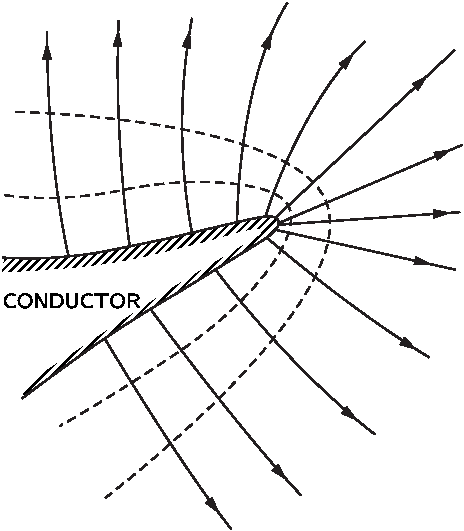
\includegraphics[width=\linewidth]{tip.pdf}
			\end{column}
		\end{columns}
	\end{onlyenv}
	\begin{onlyenv}<2>
		\begin{block}{}\justifying
			<<Іонний вітер>> --- явище, за якого рух повітря створюється за допомогою
			електричного поля.
		\end{block}
		\begin{columns}
			\begin{column}{0.6\linewidth}
				\begin{block}{}\justifying
					Наявні в повітрі в невеликій кількості вільні заряди (іони обох знаків і електрони)
					поблизу вістря розганяються сильним полем і, вдаряючись об атоми газу, іонізують
					їх. Створюється область просторового заряду, звідки іони того ж знака, що й вістря,
					виштовхуються полем, захоплюючи за собою атоми газу. Потік атомів та іонів,
					спрямований від вістря, створює враження <<стікання зарядів>>.
					%  При цьому вістря розряджається (іонами протилежного знака, що потрапляють на
					%нього) і одночасно отримує імпульс, спрямований проти стікання.
				\end{block}
			\end{column}
			\begin{column}{0.4\linewidth}\centering
				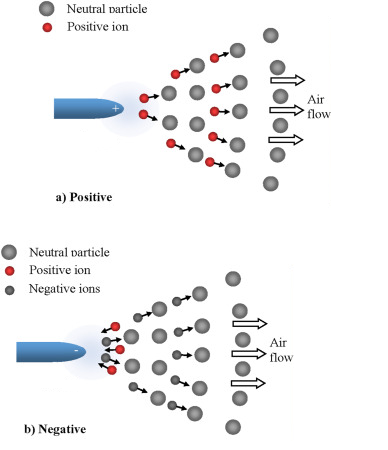
\includegraphics[width=0.9\linewidth]{ion_wind}
			\end{column}
		\end{columns}
		\begin{block}{}
			\href{https://www.youtube.com/watch?v=LNobNwDX2jQ}{Відео: Демонстрація іонного вітру}
		\end{block}
	\end{onlyenv}
\end{frame}
% ===========================================================================



%% --------------------------------------------------------
\section{Єдиність розв'язку електростатичної задачі}
%% --------------------------------------------------------



% ===========================================================================
\begin{frame}{Рівняння Пуассона та Лапласа}{Єдиність розв'язку електростатичної задачі}
	\begin{block}{}\justifying
		Задача електростатики зводиться до \alert{знаходження розв'язку}
		рівняння Пуассона $\tcbhighmath{\nabla^2\phi = - 4\pi\rho}$ (або Лапласа
		$\tcbhighmath{\nabla^2\phi = 0}$).
	\end{block}
	\begin{block}{}\justifying
		Розв'язок задачі можна \alert{вгадати}! Якщо \alert{вгаданий розв'язок} задачі в деякій
		\alert{області} задовольняє рівнянню Лапласа (або Пуассона)  і задовольняє \alert{умовам на
			границі області}, то він буде правильним і \alert{єдиним}, незважаючи на те, що ми його
		вгадали. Це твердження грунтується на \alert{теоремі єдиності}.
	\end{block}


	\begin{block}{}\justifying\footnotesize
		Дійсно, якщо при заданій конфігурації зарядів і потенціалів
		на границях розв'язок не один, то буде різний електричний <<ландшафт>>, отже, у кожній
		точці поле $\Efield$, узагалі кажучи, буде неоднозначним --- що є фізичного абсурдним.
	\end{block}

	\begin{block}{}\justifying
		Використання теореми єдиності дуже \alert{спрощує} розв'язання деяких електростатичних
		задач.
	\end{block}

\end{frame}
% ===========================================================================



%% --------------------------------------------------------
\section{Метод електричних зображень}
%% --------------------------------------------------------



% ============================== Слайд ## ===================================
\begin{frame}{Метод електричних зображень}{Ідея методу на прикладі заземленої площини}
	\begin{onlyenv}<1>
		\begin{block}{}\justifying
			Метод \alert{грунтується на теоремі єдиності} і \alert{полягає у вгадуванні
				конфігурації зарядів}, у якій поле в цікавій для нас частині простору було б тим же
			самим, які і у розглядуваної задачі.
		\end{block}
	\end{onlyenv}
	\begin{onlyenv}<1>
		\begin{block}{}\justifying\small
			Розглянемо ідею цього методу на прикладі, коли точковий заряд $q$
			знаходиться	біля нескінченної заземленої провідної площини.
		\end{block}
		\begin{center}
			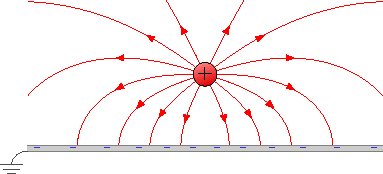
\includegraphics[width=6cm]{charge_near_plane.pdf}
		\end{center}
		\begin{alertblock}{}
			Як знайти поле у верхній частині простору? Як знайти розподіл заряду на площині?
		\end{alertblock}
	\end{onlyenv}
	\begin{overprint}
		\onslide<2>
		\begin{alertblock}{}
			Як знайти поле у верхній частині простору? Як знайти розподіл заряду на площині?
		\end{alertblock}
		\onslide<3>
		\begin{alertblock}{}
			Можна вгадати таку конфігурацію зарядів, у якої буде еквіпотенціальна поверхня, на якій
			$\phi = 0$!
		\end{alertblock}
		\onslide<4>
		\begin{block}{}\justifying
			Для обчислення поля достатньо ввести \alert{фіктивний заряд-зображення $q' = -q$},
			помістивши його по інший бік площини на такій самій відстані від неї, що й заряд $q$.
			Фіктивний заряд $q'$ створює у верхньому півпросторі точно таке саме поле, як і індуковані
			заряди на площині.
		\end{block}
	\end{overprint}

	\begin{overprint}
		\onslide<2>
		\begin{center}
			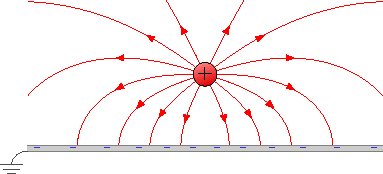
\includegraphics[width=6cm]{charge_near_plane.pdf}
		\end{center}
		\onslide<3>
		\begin{center}
			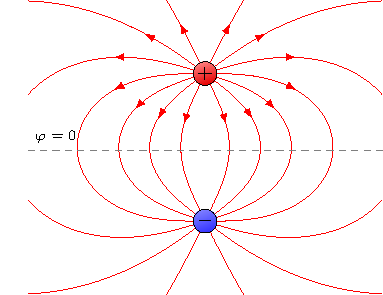
\includegraphics[width=6cm]{two_charges.pdf}
		\end{center}
		\onslide<4>
		\begin{center}
			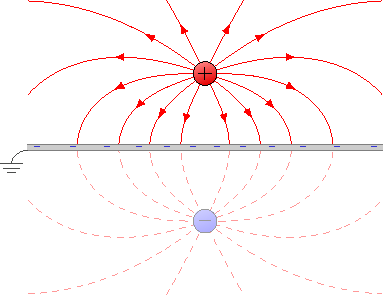
\includegraphics[width=6cm]{charge_image.pdf}
		\end{center}
	\end{overprint}
\end{frame}
% ===========================================================================



% ============================== Слайд ## ===================================
\begin{frame}{Задача}{}
       \begin{exampleblock}{Задача }
            Знайдіть з якою густиною заряд розподіляється по поверхні металевої пластини
            $\sigma(x)$, де $x$ --- координата вздовж пластини, за $x = 0$ покладіть положення
            навпроти заряду.
        \end{exampleblock}
		\begin{center}
			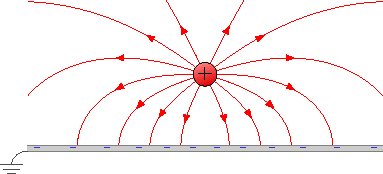
\includegraphics[width=6cm]{charge_near_plane.pdf}
		\end{center}
\end{frame}
% ===========================================================================



% ============================== Слайд ## ===================================
\begin{frame}{Метод електричних зображень}{Заряд поблизу сферичної поверхні}
	\begin{overprint}
		\onslide<1>
		\begin{block}{}\justifying
			В системі двох різнойменних зарядів знайдуться сферичні еквіпотенціальні поверхні. На
			одній з таких поверхонь потенціал дорівнює $\phi = 0$.
		\end{block}
		\onslide<2>
		\begin{block}{}\justifying
			Якщо заряд $q$ опиниться поблизу \alert{незарядженої} і \alert{заземленої провідної сфери} і
			треба знайти поле поза сферою, то треба підібрати положення і величину заряду зображення $q'$,
			щоб задовольнити теоремі єдиності.
		\end{block}
		\onslide<3>
		\begin{block}{}\justifying
			Величина заряду $q'$ і його положення $a$ по відношенню до центра сфери дається формулами:
			\begin{equation*}
				a = \frac{R^2}{b}, \quad   q' = -\frac{R}{b}q.
			\end{equation*}
		\end{block}
		\onslide<4>
		\begin{block}{}\justifying
			Якщо сфера \alert{ізольована} і \alert{несе заряд $q_0$}, то зображення утворюється
			двома зарядами: перший $q' $перебуває на відстані $a$ від центру сфери і додається
			другий заряд-зображення $q''$, який знаходиться в центрі сфери і має величину таку, що:
			\begin{equation*}
				q' + q'' = q_0.
			\end{equation*}
		\end{block}
	\end{overprint}
	\begin{overprint}
		\onslide<1>
		\begin{center}
			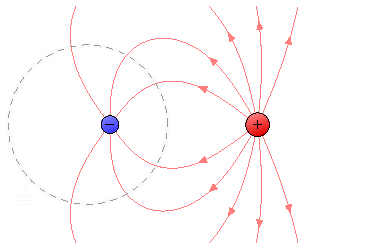
\includegraphics[page=1]{mirrorsphere}
		\end{center}
		\onslide<2>
		\begin{center}
			\includegraphics[page=2]{mirrorsphere}
		\end{center}
		\onslide<3>
		\begin{center}
			\includegraphics[page=3]{mirrorsphere}
		\end{center}
		\onslide<4>
		\begin{center}
			\includegraphics[page=4]{mirrorsphere}
		\end{center}
	\end{overprint}
\end{frame}
% ===========================================================================




% ============================== Слайд ## ===================================
\begin{frame}{Задачі}{}

    \begin{onlyenv}<1>
        \begin{exampleblock}{Задача 1}\justifying
            Знайдіть потенціал \alert{незарядженої} і \alert{незаземленої} металевої сфери радіуса $R$,
            що знаходиться в полі заряду $q$, який розташований на відстані $b$ ($b > R$) від центра кулі.
        \end{exampleblock}
    \end{onlyenv}

	\begin{onlyenv}<2>

		%=========================================================
		\begin{exampleblock}{Задача 2}\label{prb:3spheres_middle_ground}\justifying
			Три концентричні сфери мають радіуси $R_1$, $R_2$ та $R_3$ ($R_1 <R_2 < R_3$). Сфери $1$ та
			$3$ несуть заряди відповідно $+Q$ і $-Q$. Середня сфера $2$ заземлена провідником
			(рис.). Знайти заряд $q$ заземленої сфери $2$ та залежності
			$E(r)$ та $\phi(r)$ і побудувати їх графіки.

			\medskip

			Відповідь: $q=Q\left( \frac{R_2}{R_3} - 1\right) $

			\begin{figure}[h!]\centering
				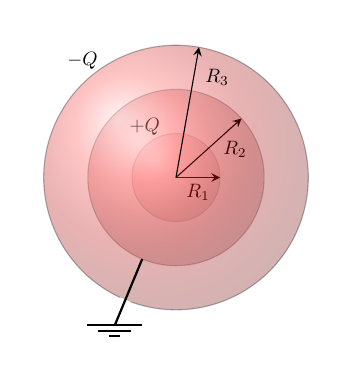
\begin{tikzpicture}[scale=0.7, transform shape]
					\def\R{0.8}
					\draw [ball color=red, opacity=0.1] (0,0) circle (\R);
					\draw [-stealth] (0,0) -- node[below] {$R_1$} (0:\R);
					\node [above=2pt] at (135:\R) {$+Q$};
					\draw [ball color=red, opacity=0.2] (0,0) circle ({2*\R});
					\draw [-stealth](0,0) -- node[pos=0.9, below = 5pt] {$R_2$} (42:{2*\R});
					\draw [ball color=red, opacity=0.3] (250:{3*\R}) arc (250:605:{3*\R});
					\draw [-stealth](0,0) -- node[pos=0.9, below right=1pt] {$R_3$} (80:{3*\R});
					\node [above=4pt] at (135:{3*\R}) {$-Q$};
					\draw [thick] (247.5:{2*\R}) -- (247.5:{3*\R +0.5}) coordinate (G);
					\draw [thick] (G) +(-0.5,0) -- +(0.5,0)
					+(-0.3,-0.1) -- +(0.3,-0.1)
					+(-0.1,-0.2) -- +(0.1,-0.2);
				\end{tikzpicture}
				\label{3spheres_middle_ground}
			\end{figure}

		\end{exampleblock}

	\end{onlyenv}

	\begin{onlyenv}<3>
		\begin{exampleblock}{Задача 3}\justifying
			На відстані $b= 10R$ від заземленої незарядженої металевої сфери радіусом $R$ розташований
			точковий електричний диполь з моментом $p$, причому вісь диполя перпендикулярна прямій, що
			сполучає центр сфери з серединою осі диполя (рис). Знайти силу взаємодії між
			диполем і сферою.

			\medskip

			Відповідь: $F = \frac{3p^2R^3}{b^7}$, взаємодія~--- притягування.

			\begin{figure}[h!]\centering
				\begin{tikzpicture}
					\draw [ball color=gray, opacity=0.5] (0,0) circle (1);
					\draw [-latex] (4,-0.5) -- (4,0.5) node [above] {$\vect{p}$};
					\draw [-latex'] (0,0) -- node [right] {$R$}(135:1);
					\draw [latex'-latex'] (0,0) -- node [below] {$b$}(4,0);
					\draw (0,-1) -- (0,-1.5) coordinate (G);
					\draw (G) +(-0.5,0) -- +(0.5,0)
					+(-0.3,-0.1) -- +(0.3,-0.1)
					+(-0.1,-0.2) -- +(0.1,-0.2);
				\end{tikzpicture}
				\label{Ovch2.32}
			\end{figure}
		\end{exampleblock}

	\end{onlyenv}

\end{frame}
% ===========================================================================



%% --------------------------------------------------------
\section{Металева куля в однорідному полі}
%% --------------------------------------------------------


% ============================== Слайд ## ===================================
\begin{frame}{Металева куля в однорідному полі $\Efield_0$}{}
	\begin{center}
		\begin{tikzpicture}[scale=0.75, transform shape]
% ============================ ��������� ===================================
\pgfmathsetmacro{\step}{0.4}
\pgfmathsetmacro{\ea}{5}
\pgfmathsetmacro{\eb}{1}
\pgfmathsetmacro{\shape}{1}
% ============================== ������� ===================================
\draw [
    raw gnuplot, red,
    ] plot[id=curve, raw gnuplot] function {
            set isosamples 55, 55;
            set contour base;
            set cntrparam levels incremental -2.2,\step,2.2;
            %set style data lines;
            unset  surface;
            splot [-4:4] [-2.2:2.2] (y*(1+\shape/(x**2 + y**2))) ;
            };
% ================================ ���� ======================================
\fill[ball color=gray!20, draw=gray!30, thick] (0,0) circle (1.01);
% ======================= ������ �� ����� ==================================
\foreach \i in {-2.2,-1.8,...,2.2} {
\draw[red, -latex', rotate around = {{-asin(\i/(3 +\shape/3))}:({asin(\i/(3 +\shape/3))}:3)}] ({asin(\i/(3 +\shape/3))}:3) -- ({asin(\i/(3 +\shape/3))}:3.1);
\draw[red, -latex',rotate around = {{180-asin(\i/(3 +\shape/3))}:({180+asin(\i/(3 +\shape/3))}:3)} ] ({180+asin(\i/(3 +\shape/3))}:3) -- ({180+asin(\i/(3 +\shape/3))}:3.1);
}
% ============================ ����� ������ =================================
\foreach \i in {70,30,15,0}{
%==================================
\node at (\i:1.1) {\tiny $+$};
\node at (-\i:1.1) {\tiny $+$};
\node at ({180-\i}:1.1) {\tiny $-$};
\node at ({180+\i}:1.1) {\tiny $-$};
}
\end{tikzpicture}
	\end{center}
	\begin{block}{}\justifying
		Металева куля набуває дипольного моменту внаслідок 	перерозподілу зарядів по її поверхні:
		\begin{equation*}
			\vect{p} = R^3\Efield_0
		\end{equation*}
	\end{block}
	%	Потенціал кулі:
	%	\begin{equation*}
	%		\phi =
	%		\begin{cases}
	%			0,                                                                      & r \le R \\
	%			-\left( \Efield_0\cdot \vect{r}\right) + \frac{\vect{p} \vect{r}}{r^3}, & r > R
	%		\end{cases}
	%	\end{equation*}
\begin{columns}
	\begin{column}{0.5\linewidth}
	\begin{block}{}\centering
		Поле зовні та всередині кулі:
\begin{equation*}
    			\Efield =
			\begin{cases}
				0,
				        & r \le R \\
				\Efield_0 - \frac{\vect{p}}{r^3} + \frac{3\left(\vect{p}\vect{r}\right)\vect{r}
				}{r^5}, & r > R,
			\end{cases}
\end{equation*}
	\end{block}
	\end{column}
	\begin{column}{0.5\linewidth}
	\begin{block}{}\centering
		Заряди на поверхні:
        \begin{equation*}
     			\sigma = \frac{3}{4\pi} \frac{\Efield_0\vect{r}}{R}.
        \end{equation*}
	\end{block}
	\end{column}
\end{columns}

\end{frame}
% ===========================================================================




%% --------------------------------------------------------
\section{Сили, що діють на поверхню провідника в полі}
%% --------------------------------------------------------




% ============================== Слайд ## ===================================
\begin{frame}{Сили, що діють на поверхню провідника в полі}{}
	\begin{columns}
		\begin{column}{0.65\linewidth}
			\begin{block}{}\justifying
				На малий елемент $dS$ поверхні провідника діє сила:
				\begin{equation*}
					dF = dq E_0 = \sigma dS \cdot  E_0,
				\end{equation*}
				з боку \alert{поля $E_0$ інших зарядів} в місці
				знаходження заряду $dq = \sigma dS$. Але прилад може віиміряти \alert{сумарне поле
					$E$}, тобто поле  \alert{інших зарядів $E_0$} плюс \alert{власне поле
					$E_{\sigma}$}, і  розрізнити їх не може!
			\end{block}
		\end{column}
		\begin{column}{0.34\linewidth}\centering
			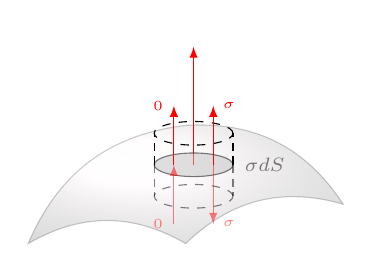
\begin{tikzpicture}[>=latex, every node/.style={font=\scriptsize},
		transform shape]
    \pgfmathsetmacro\h{0.4}
    \pgfmathsetmacro\r{0.5}
	\begin{scope}[opacity=0.2]
		\draw[ball color=red!5] (0,0) to[bend left] ++(2,1.5)  to[bend left] ++(2,-1)
		to[bend right]
		++(-2, -0.5)  to[bend
			right] cycle;

	\end{scope}

    \pgfmathsetmacro\x{2.1}
    \pgfmathsetmacro\y{1.0}
    \coordinate (A)  at (\x,          \y);
    \coordinate (A1) at ({\x - \r},   \y);
    \coordinate (A2) at ({\x + \r},   \y);
    \coordinate (E0) at ({\x - \r/2}, \y);
    \coordinate (Es) at ({\x + \r/2}, \y);

	\draw[->, red]  (A) -- ++(90:1.5) coordinate (B)
	node[above] {$\Efield$};

	\draw[fill=gray!50, opacity=0.5] (A) circle[x radius =\r, y radius= 0.15] node[right=15pt]
	{$\sigma dS$};
	\draw[dashed] (A) ++(90:\h) circle[x radius =\r, y radius= 0.15];

	\draw[densely dashed] (A1) -- ++(90:\h);
	\draw[densely dashed] (A2) -- ++(90:\h);

    \draw[->, red] (Es) -- ++(0,+0.75) node[right] {$\Efield_{\sigma}$};
    \draw[->, red] (E0) -- ++(0,+0.75) node[left] {$\Efield_{0}$};

    \begin{scope}[opacity=0.5]
        \draw[densely dashed] (A1) -- ++(90:-\h);
   		\draw[densely dashed] (A2) -- ++(90:-\h);
        \draw[dashed] (A) ++(90:-\h) circle[x radius =\r, y radius= 0.15];

        \draw[->, red] (Es) -- ++(0,-0.75) node[right] {$\Efield_{\sigma}$};
        \draw[<-, red] (E0) -- ++(0,-0.75) node[left] {$\Efield_{0}$};
    \end{scope}

\end{tikzpicture}
		\end{column}
	\end{columns}
	\begin{overprint}
		\onslide<1>
		\begin{alertblock}{}\justifying
			Задача 	полягає в тому, щоб виразити силу саме через сумарне поле.
		\end{alertblock}
		\onslide<2>
		\begin{block}{}\justifying
			Оскільки поле в середині провідника  $E = 0$, то власне поле за модулем має дорівнювати
			полю <<чужих>> зарядів:
			\begin{equation*}
				E_0 = E_{\sigma},
			\end{equation*}
			це означає, що \alert{густина заряду підлаштовується під зовнішнє поле}!
		\end{block}
		\onslide<3>
		\begin{block}{}\justifying
			Гранична умова дає поле у вакуумі:
			\begin{equation*}
				E = E_0 + E_{\sigma} = 2 E_0 = 4\pi\sigma.
			\end{equation*}
		\end{block}
%		\onslide<3>
		\begin{block}{}\justifying
			Сила, що діє на одиницю поверхні провідника
			\begin{equation*}
				\frac{dF}{dS} = f = \frac12 \sigma E = \frac{E^2}{8\pi}.
			\end{equation*}
		\end{block}
	\end{overprint}
\end{frame}
% ===========================================================================



% ============================== Слайд ## ===================================
\begin{frame}{Задачі}{}
	\begin{exampleblock}{Задача 1}\justifying
		Знайдіть силу взаємодії двох заряджених металевих пластин, що знаходяться на малій відстані
		одна від одної. Густина заряду кожної з пластин $\sigma$. Площа пластин $S$.

		\medskip

		Якщо пластини мають форму дисків радіуса $R$. Чому буде дорівнювати сила взаємодії між ними на
		відстані $\ell \gg R$?
	\end{exampleblock}


	\begin{exampleblock}{Задача 2}\justifying
		Металева сфера радіуса $R$ складена з двох півсфер. Визначити силу $F$, з якою відштовхуються
		ці півсфери, якщо повний заряд сфери дорівнює~$Q$.

		\bigskip

		Відповідь: $F= \frac{Q^2}{8R^2}$.
	\end{exampleblock}
\end{frame}
% ===========================================================================




%% --------------------------------------------------------
\section*{{Підсумки}}
%% --------------------------------------------------------



% ============================== Слайд ## ===================================
\begin{frame}{Підсумки}{}
\begin{enumerate}
\item В стаціонарному стані в об'ємі провідника результуюче електричне поле $\Efield = 0$.
\item В об'ємі провідника зарядів нема $\rho = 0$ (заряди розташовуються на поверхні провідника).
\item Поле біля поверхні провідника $E_n = 4\pi\sigma$, $E_{\tau} = 0$.
\item Поверхня провідника є еквіпотенціальною поверхнею! Потенціал в об'ємі провідника
постійний і дорівнює потенціалу на його поверхні.
\item Сила, що діє на поверхню провідника в електричному полі $f = \frac{E^2}{8\pi}$.
\end{enumerate}
\end{frame}
% ===========================================================================


\end{document}
